\documentclass[12pt,a4paper]{article}

\usepackage[utf8]{inputenc}
\usepackage[T2A]{fontenc}
\usepackage[ukrainian]{babel}
\usepackage{geometry}
\geometry{
    left=2cm,
    right=2cm,
    top=2cm,
    bottom=2cm
}

\usepackage[table]{xcolor}
\usepackage{amsmath}
\usepackage{graphicx}
\usepackage{subcaption}
\usepackage{multirow}
\usepackage{makecell}
\usepackage{pdflscape}
\usepackage{array}
\newcolumntype{C}[1]{>{\centering\arraybackslash}m{#1}}

\usepackage[
  unicode,
  pdftitle={ІО-41, Давидчук А.М., АК. Частина 1, Лабораторна робота №1},
  pdfauthor={Давидчук Артем},
  pdfsubject={Архітектура Комп'ютерів. Частина 1}
]{hyperref}

\begin{document}

    \begin{titlepage}

        \begin{center}
\includegraphics[width=0.7\textwidth]{../../../TITLES/letterhead.png}\end{center}

        \begin{center}
            \large Національний технічний університет України\\
            «Київський політехнічний інститут імені Ігоря Сікорського»\\[1em]
            Факультет інформатики та обчислювальної техніки\\
            Кафедра обчислювальної техніки
        \end{center}

        \vfill

        \begin{center}
            \textbf{\LARGE Архітектура Комп'ютерів. Частина 1}\\[2em]
            \textbf{\Large Лабораторна робота №1}\\[0.5em]
            «Синтез арифметико-логічних пристроїв з розподіленою логікою» 
        \end{center}

        \vfill

        \begin{flushright}
            Виконав: студент 2 курсу ФІОТ, гр. ІО-41\\
            \textit{Давидчук А. М.}\\
            Залікова книжка № 4106\\[1em]
            Перевірив: \textit{Верба О.\,А.}
        \end{flushright}

        \vfill

        \begin{center}Київ --- 2026\end{center}

    \end{titlepage}

    \noindent
    \textbf{\underline{Тема:}} «Синтез арифметико-логічних пристроїв з розподіленою логікою» .

    \vspace{1em}

    \noindent
    \textbf{\underline{Мета:}} одержати навички в проектуванні арифметико-логічних пристроїв з розподіленою логікою і автоматів управління з жорсткою логікою

    \begin{center} \textbf{\large Порядок виконання роботи} \end{center}

    \begin{enumerate}
        \item Варіанти завдання визначаються молодшими розрядами $a_7,\ldots,a_1$ двійкового номера залікової книжки студента відповідно з табл.~2.7--2.9 у методичних вказівках. Множення 1-м способом виконати в доповняльному коді (ДК) для чисел із знаками. Для інших функцій операнди є додатні числа.

        \item Розробити операційну схему пристрою та змістовний мікроалгоритм обчислення функції (виконання операції множення) відповідно з табл.~2.7 у методичних вказівках.

        \item Розробити функціональну схему операційного пристрою. Для побудови схеми можна використовувати комбінаційний суматор, регістр-лічильник циклів та асинхронні регістри, що мають входи управління зсувами і занесенням інформації. На схемі повинні бути зазначені розрядність регістрів та шин.

        \item Виконати логічне моделювання роботи операційного пристрою за допомогою таблиці станів регістрів та лічильника. Задати самостійно значення операндів (3 -- 4 розряди).

        \item Здійснити синтез пристрою управління, тип тригерів і управляючого автомату обрати із табл.~2.8 та 2.9 у методичних вказівках. Ураховувати, що мікрооперації на регістрах виконуються за перепадом управляючих сигналів з $1$ в $0$.
    
        \item В моделюючій програмі ПРОГМОЛС~2.0 (AFDK) побудувати схему операційного пристрою для множення чисел або обчислення функції та доповнити її схемою управляючого автомата. На першому етапі виходи автомата до входів операційного пристрою не підключати. Налагодити окремо схему операційного пристрою та схему управляючого автомата.

        \item Підключити до управляючих входів операційного пристрою виходи автомата. Зробити комплексне налагодження схеми і переконатися в правильності одержаних результату.

        \item Перейти до асинхронного моделювання. Дослідити зазначені викладачем часові параметри схеми.

    \end{enumerate}

    \begin{center} \textbf{\large Хід роботи} \end{center}

    Мій номер залікової книжки: 4106, що у двіковому вигляді є 0001 0000 0000 1010.
    Звідси $a_7 = 0, a_6 = 0, a_5 = 0, a_4 = 1, a_3 = 0, a_2 = 1, a_1 = 0$.

    \vspace{1em}

    Звідси мій варіант завдання: \underline{Множення, 2 способом}. Тобто обчислити функцію

    \[
    C = A \, B
    \]

    де $A$ та $B$ -- правильні додатні дроби, а $C$ -- результат множення.

    \vspace{1em}

    Мій тип тригера: \underline{T тригер}.

    \vspace{1em}

    Мій тип автомата: \underline{Мілі}.

    \newpage

    \noindent
    Операційна схема множення за 2 способом для 4 розрядних вхідних операндів $A$ та $B$:

    \begin{figure}[h!]
        \centering
        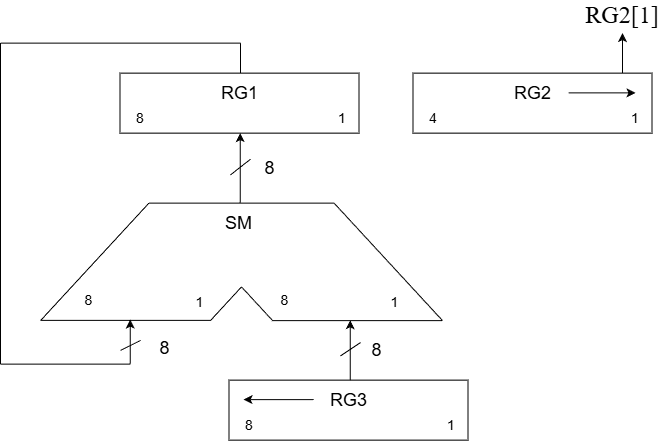
\includegraphics[width=0.7\linewidth]{media/png files/op.png}
        \caption{Операційна схема множення за 2 способом для 4 розрядних операндів}
    \end{figure}

    \noindent
    Функціональний мікроалгоритм множення за 2 способом для 4 розрядних операндів:

    \begin{figure}[h!]
        \centering
        
\includegraphics[width=0.57 \linewidth]{media/png files/alg.png}
        \caption{\centering Функціональний мікроалгоритм множення за 2 способом для 4 розрядних вхідних операндів $A$ та $B$}
    \end{figure}

    \noindent
    Проведемо демонстрацію множення довільних чисел $A$ та $B$ таблицею станів регістрів:

    \vspace{1em}

    \noindent
    Нехай

    $A = 0{,}1011 = 11$, $B = 0{,}1000 = 8$, звідси $C = A \, B = 11 \cdot 8 = 88 = 0{,}0101 \, 1000$. Перевіримо:

    \begin{table}[h!]

        \begin{tabular}{|c|c|c|c|p{7.5cm}|}
        \hline
        \textbf{№} &
        \makecell{\textbf{RG3} \\ \\ 8 \qquad \empty \quad 1} &    % <-- Одна комірка замість двох
        \makecell{\textbf{RG2} \\ \\ 4 \qquad \empty \quad 1} &
        \makecell{\textbf{RG1} \\ \\ 8 \qquad \quad \empty \qquad 1} &
        \textbf{Мікрооперації} \\
        \hline
        \textbf{--} & 00001000 & 101\textbf{1} & 00000000 &
        \makecell[l]{\texttt{RG3 = 0..0.B; RG2 = A; RG1 = 0;}}\\
        \hline
        \textbf{1} &
        \makecell{00001000\\[1em] \textit{Після зсуву:}\\ 00010000} &
        \makecell{1011\\[1em] \textit{Після зсуву:}\\ 010\textbf{1}} &
        \makecell[l]{
        \(
        \begin{array}{r} % r - вирівнюємо вправо для акуратності
        00000000 \\
        \ + \ 00001000 \\
        \hline
        00001000
        \end{array}
        \)
        } &
        \makecell[l]{\texttt{RG1 := RG1 + RG3;} \\
        \texttt{RG3 := l(RG3).0; RG2 := 0.r(RG2);}} \\
        \hline
        \textbf{2} &
        \makecell{00010000\\[1em] \textit{Після зсуву:}\\ 00100000} & 
        \makecell{0101\\[1em] \textit{Після зсуву:}\\ 001\textbf{0}} &
        \makecell[l]{
        \(
        \begin{array}{r} % r - вирівнюємо вправо для акуратності
        00001000 \\
        \ + \ 00010000 \\
        \hline
        00011000
        \end{array}
        \)
        } &
        \makecell[l]{\texttt{RG1 := RG1 + RG3;} \\
        \texttt{RG3 := l(RG3).0; RG2 := 0.r(RG2);}} \\
        \hline
        \textbf{3} &
        \makecell{00100000\\[1em] \textit{Після зсуву:}\\ 01000000} & 
        \makecell{0010\\[1em] \textit{Після зсуву:}\\ 000\textbf{1}}
        & 00011000 &
        \texttt{RG3 := l(RG3).0; RG2 := 0.r(RG2);} \\
        \hline
        \textbf{4} &
        \makecell{01000000\\[1em] \textit{Після зсуву:}\\ 10000000} & 
        \makecell{0001\\[1em] \textit{Після зсуву:}\\ \textbf{0000}} &
        \makecell[l]{
        \(
        \begin{array}{r} % r - вирівнюємо вправо для акуратності
        00011000 \\
        \ + \ 01000000 \\
        \hline
        01011000
        \end{array}
        \)
        } &
        \makecell[l]{\texttt{RG1 := RG1 + RG3;} \\
        \texttt{RG3 := l(RG3).0; RG2 := 0.r(RG2);}} \\
        \hline

        \end{tabular}

        \caption{Таблиця станів регістрів при множенні}

    \end{table}

    \noindent
    Регістр \texttt{RG2} став нульовим, що свідчить про закінчення операції множення, і в регістрі \texttt{RG1} записана відповідь, а саме: 0,0101\,1000 що співпадає із раніше вручну
    обчисленим значенням, що свідчить про коректність виконання алгоритму множення 2 способом.

    \newpage

    \noindent
    Функціональна схема виконання множення:

    \begin{figure}[h!]
        \centering
        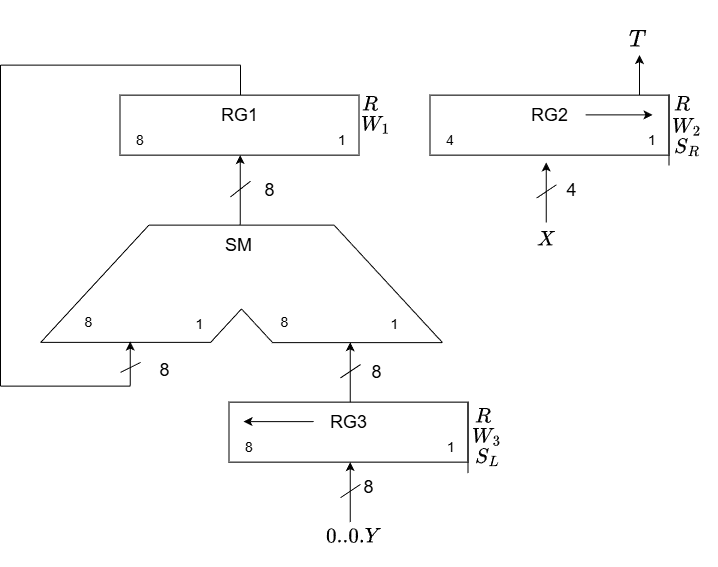
\includegraphics[width=0.7\linewidth]{media/png files/func.png}
        \caption{\centering Функціональна схема множення за 2 способом для 4 розрядних вхідних операндів $A$ та $B$}
    \end{figure}

    \noindent
    Таблиця управляючих сигналів:

    \begin{table}[h!]
        \centering
        \renewcommand{\arraystretch}{1.2}
        \setlength{\tabcolsep}{10pt}

        \begin{tabular}{|c|l|c|}
            \hline
            \textbf{Вузол} & \textbf{Мікрооперація} & \textbf{Управляючий сигнал} \\
            \hline

            \multirow{2}{*}{RG1} & Запис       & $W_{1}$  \\ \cline{2-3}
                                & Скидання & $R$ \\ \hline

            \multirow{3}{*}{RG2} & Запис                 & $W_{2}$ \\ \cline{2-3}
                                & Скидання & $R$     \\ \cline{2-3}
                                & Зсув праворуч & $S_R$     \\ \hline

            \multirow{3}{*}{RG3} & Запис                 & $W_{3}$ \\ \cline{2-3}
                                & Скидання & $R$     \\ \cline{2-3}
                                & Зсув ліворуч & $S_L$     \\ \hline
        \end{tabular}

        \caption{Таблиця мікрооперацій та управляючий сигналів}

    \end{table}

    \newpage

    \noindent
    Звичайний та закодований структурні мікроалгоритми множення 2 способом:

    \begin{figure}[h!]
        \centering

        \begin{subfigure}[t]{0.48\textwidth}
            \centering
            
\includegraphics[width=1.0\linewidth]{media/png files/alg1.png}
            \subcaption*{а)}
        \end{subfigure}
        \hfill
        \begin{subfigure}[t]{0.48\textwidth}
            \centering
            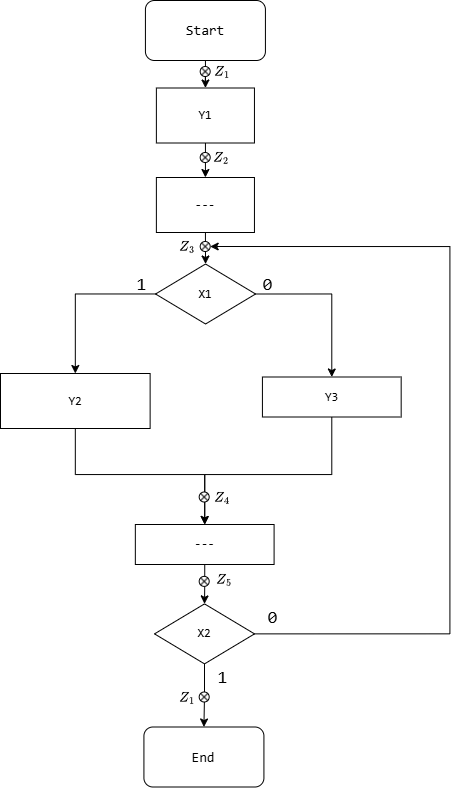
\includegraphics[width=0.9\linewidth]{media/png files/alg2.png}
            \subcaption*{б)}
        \end{subfigure}

        \caption{Звичайний (а) та закодований (б) структурні мікроалгоритми множення}
    \end{figure}

    Примітка: сигнал $R$ буде подаватись поза алгоритмом вручну користувачем, тому він не входить у кодування керуючих сигналів.

    \newpage

    \noindent
    Таблиця кодування керуючих сигналів та логічних умов:

    \begin{table}[h!]
        \centering
        \renewcommand{\arraystretch}{1.2}
        \setlength{\tabcolsep}{12pt}

        \begin{tabular}{|c|c|}
            \hline
            $Y_1$ & $W_1,\, W_2,\, W_3$ \\
            \hline
            $Y_2$ & $W_1$ \\
            \hline
            $Y_3$ & $S_R,\, S_L$ \\
            \hline
            \empty & \empty \\
            \hline
            $X_1$ & \texttt{RG2[1]} ($T$) \\
            \hline
            $X_2$ & \texttt{RG2 == 0} \\
            \hline
        \end{tabular}
        \caption{Таблиця кодування керуючих сигналів та логічних умов}
    \end{table}

    На цьому етапі ми закінчили проектування операційної схеми множення 2 способом -- залишилось лише побудувати схему цього операційного пристрою.

    Далі почнемо синтез управляючого автомата, а саме синтез абстрактного та структурного. Побудуємо граф законодованого мікроалгоритма операційного пристрою:

    \begin{figure}[h!]
        \centering
        
\includegraphics[width=0.7\linewidth]{media/png files/graph.png}
        \caption{\centering Функціональна схема множення за 2 способом для 4 розрядних вхідних операндів $A$ та $B$}
    \end{figure}

    \newpage

    Тут стани $A_i$ -- додаткові стані, задля забезпечення кодування станів за кодом Грея.

    \begin{table}[h!]
        \centering
        \renewcommand{\arraystretch}{1.2}
        \setlength{\tabcolsep}{12pt}

        \begin{tabular}{|c|c|c|c|}
            \hline
            \empty & $Q_3$ & $Q_2$ & $Q_1$ \\
            \hline
            $Z_1$ & 0 & 0 & 0\\
            \hline
            $Z_2$ & 0 & 0 & 1\\
            \hline
            $Z_3$ & 1 & 0 & 1\\
            \hline
            $Z_4$ & 1 & 0 & 0\\
            \hline
            $Z_5$ & 1 & 1 & 0\\
            \hline
            $A_1$ & 0 & 1 & 0\\
            \hline
            $A_2$ & 1 & 1 & 1\\
            \hline
        \end{tabular}
        \caption{Таблиця кодування станів}
    \end{table}

    Тепер зробимо синтез структурного автомата.

    \begin{table}[h!]
        \centering
        \renewcommand{\arraystretch}{1.2}
        \setlength{\tabcolsep}{3pt}

        \resizebox{\textwidth}{!}{%
            \begin{tabular}{|
                >{\centering\arraybackslash}p{0.9cm}|
                *{3}{>{\centering\arraybackslash}p{0.9cm}|} % Код ПС: Q3 Q2 Q1
                >{\centering\arraybackslash}p{0.9cm}|
                *{3}{>{\centering\arraybackslash}p{0.9cm}|} % Код СП: Q3 Q2 Q1
                *{2}{>{\centering\arraybackslash}p{0.9cm}|} % Логічні умови: X2 X1
                *{3}{>{\centering\arraybackslash}p{0.9cm}|} % Керуючі сигнали: Y1..Y3
                *{3}{>{\centering\arraybackslash}p{0.9cm}|} % Функції: T3 T2 T1
                }
                \hline
                \multirow{2}{*}{\textbf{ПС}} &
                \multicolumn{3}{c|}{\textbf{Код ПС}} &
                \multirow{2}{*}{\textbf{СП}} &
                \multicolumn{3}{c|}{\textbf{Код СП}} &
                \multicolumn{2}{c|}{\makecell[c]{\textbf{Логічні}\\\textbf{умови}}} &
                \multicolumn{3}{c|}{\textbf{Керуючі сигнали}} &
                \multicolumn{3}{c|}{\makecell[c]{\textbf{Функції збудження}\\\textbf{тригерів}}} \\
                \cline{2-4}\cline{6-8}\cline{9-10}\cline{11-13}\cline{14-16}
                & $Q_3$ & $Q_2$ & $Q_1$ &
                & $Q_3$ & $Q_2$ & $Q_1$ &
                $X_2$ & $X_1$ &
                $Y_1$ & $Y_2$ & $Y_3$ &
                $T_3$ & $T_2$ & $T_1$ \\
                \hline

                % ---- приклад правильного рядка (16 клітинок = 15 "&") ----
                % ПС    Q3  Q2  Q1  СП      Q3  Q2  Q1 X2   X1  Y1  Y2  Y3    T3  T2  T1
                $Z_1$ & 0 & 0 & 0 & $Z_2$ & 0 & 0 & 1 & - & - & 1 & 0 & 0   & 0 & 0 & 1 \\
                $Z_2$ & 0 & 0 & 1 & $Z_3$ & 1 & 0 & 1 & - & - & 0 & 0 & 0   & 1 & 0 & 0 \\
                $Z_3$ & 1 & 0 & 1 & $Z_4$ & 1 & 0 & 0 & - & 0 & 0 & 0 & 1   & 0 & 0 & 1 \\
                $Z_3$ & 1 & 0 & 1 & $Z_4$ & 1 & 0 & 0 & - & 1 & 0 & 1 & 0   & 0 & 0 & 1 \\
                $Z_4$ & 1 & 0 & 0 & $Z_5$ & 1 & 1 & 0 & - & - & 0 & 0 & 0   & 0 & 1 & 0 \\
                $Z_5$ & 1 & 1 & 0 & $A_2$ & 1 & 1 & 1 & 0 & - & 0 & 0 & 0   & 0 & 0 & 1 \\
                $Z_5$ & 1 & 1 & 0 & $A_1$ & 0 & 1 & 0 & 1 & - & 0 & 0 & 0   & 1 & 0 & 0 \\
                $A_1$ & 0 & 1 & 0 & $Z_1$ & 0 & 0 & 0 & - & - & 0 & 0 & 0   & 0 & 1 & 0 \\
                $A_2$ & 1 & 1 & 1 & $Z_3$ & 1 & 0 & 1 & - & - & 0 & 0 & 0   & 0 & 1 & 0 \\

                \hline

            \end{tabular}%
        }
        \caption{Структурна таблиця керуючого автомата}
    \end{table}

    \noindent
    Звідси маємо такі керуючі функції та функції збудження тригерів:

    \vspace{1em}

    $Y_1 = \overline{Q_3} \, \overline{Q_2} \, \overline{Q_1}$

    \vspace{1em}

    $Y_2 = Q_3 \overline{Q_2} \, Q_1 \, X_1$

    \vspace{1em}

    $Y_3 = Q_3 \, \overline{Q_2} \, Q_1 \, \overline{X_1}$

    \vspace{1em}

    $T_3 = \overline{Q_3} \, \overline{Q_2} \, Q_1 \vee Q_3 \, Q_2 \, \overline{Q_1} \, X_2$

    \vspace{1em}

    $T_2 = Q_3 \, \overline{Q_2} \, \overline{Q_1} \vee \overline{Q_3} \, Q_2 \, \overline{Q_1} \vee Q_3 \, Q_2 \, Q_1$

    \vspace{1em}

    $T_1 = \overline{Q_3} \, \overline{Q_2} \, \overline{Q_1} \vee Q_3 \, \overline{Q_2} \, Q_1 \, \overline{X_1} \vee Q_3 \, \overline{Q_2} \, Q_1 \, X_1 \vee Q_3 \, Q_2 \, \overline{Q_1} \, \overline{X_2}$

    \vspace{1em}

    \newpage

    \noindent
    Проведемо мінімізацію всіх функцій збудження тригерів за допомогою діаграм Вейча:

    \vspace{1em}

    \begin{figure}[h!]
        \centering

        \begin{subfigure}[t]{0.3\textwidth}
            \centering
            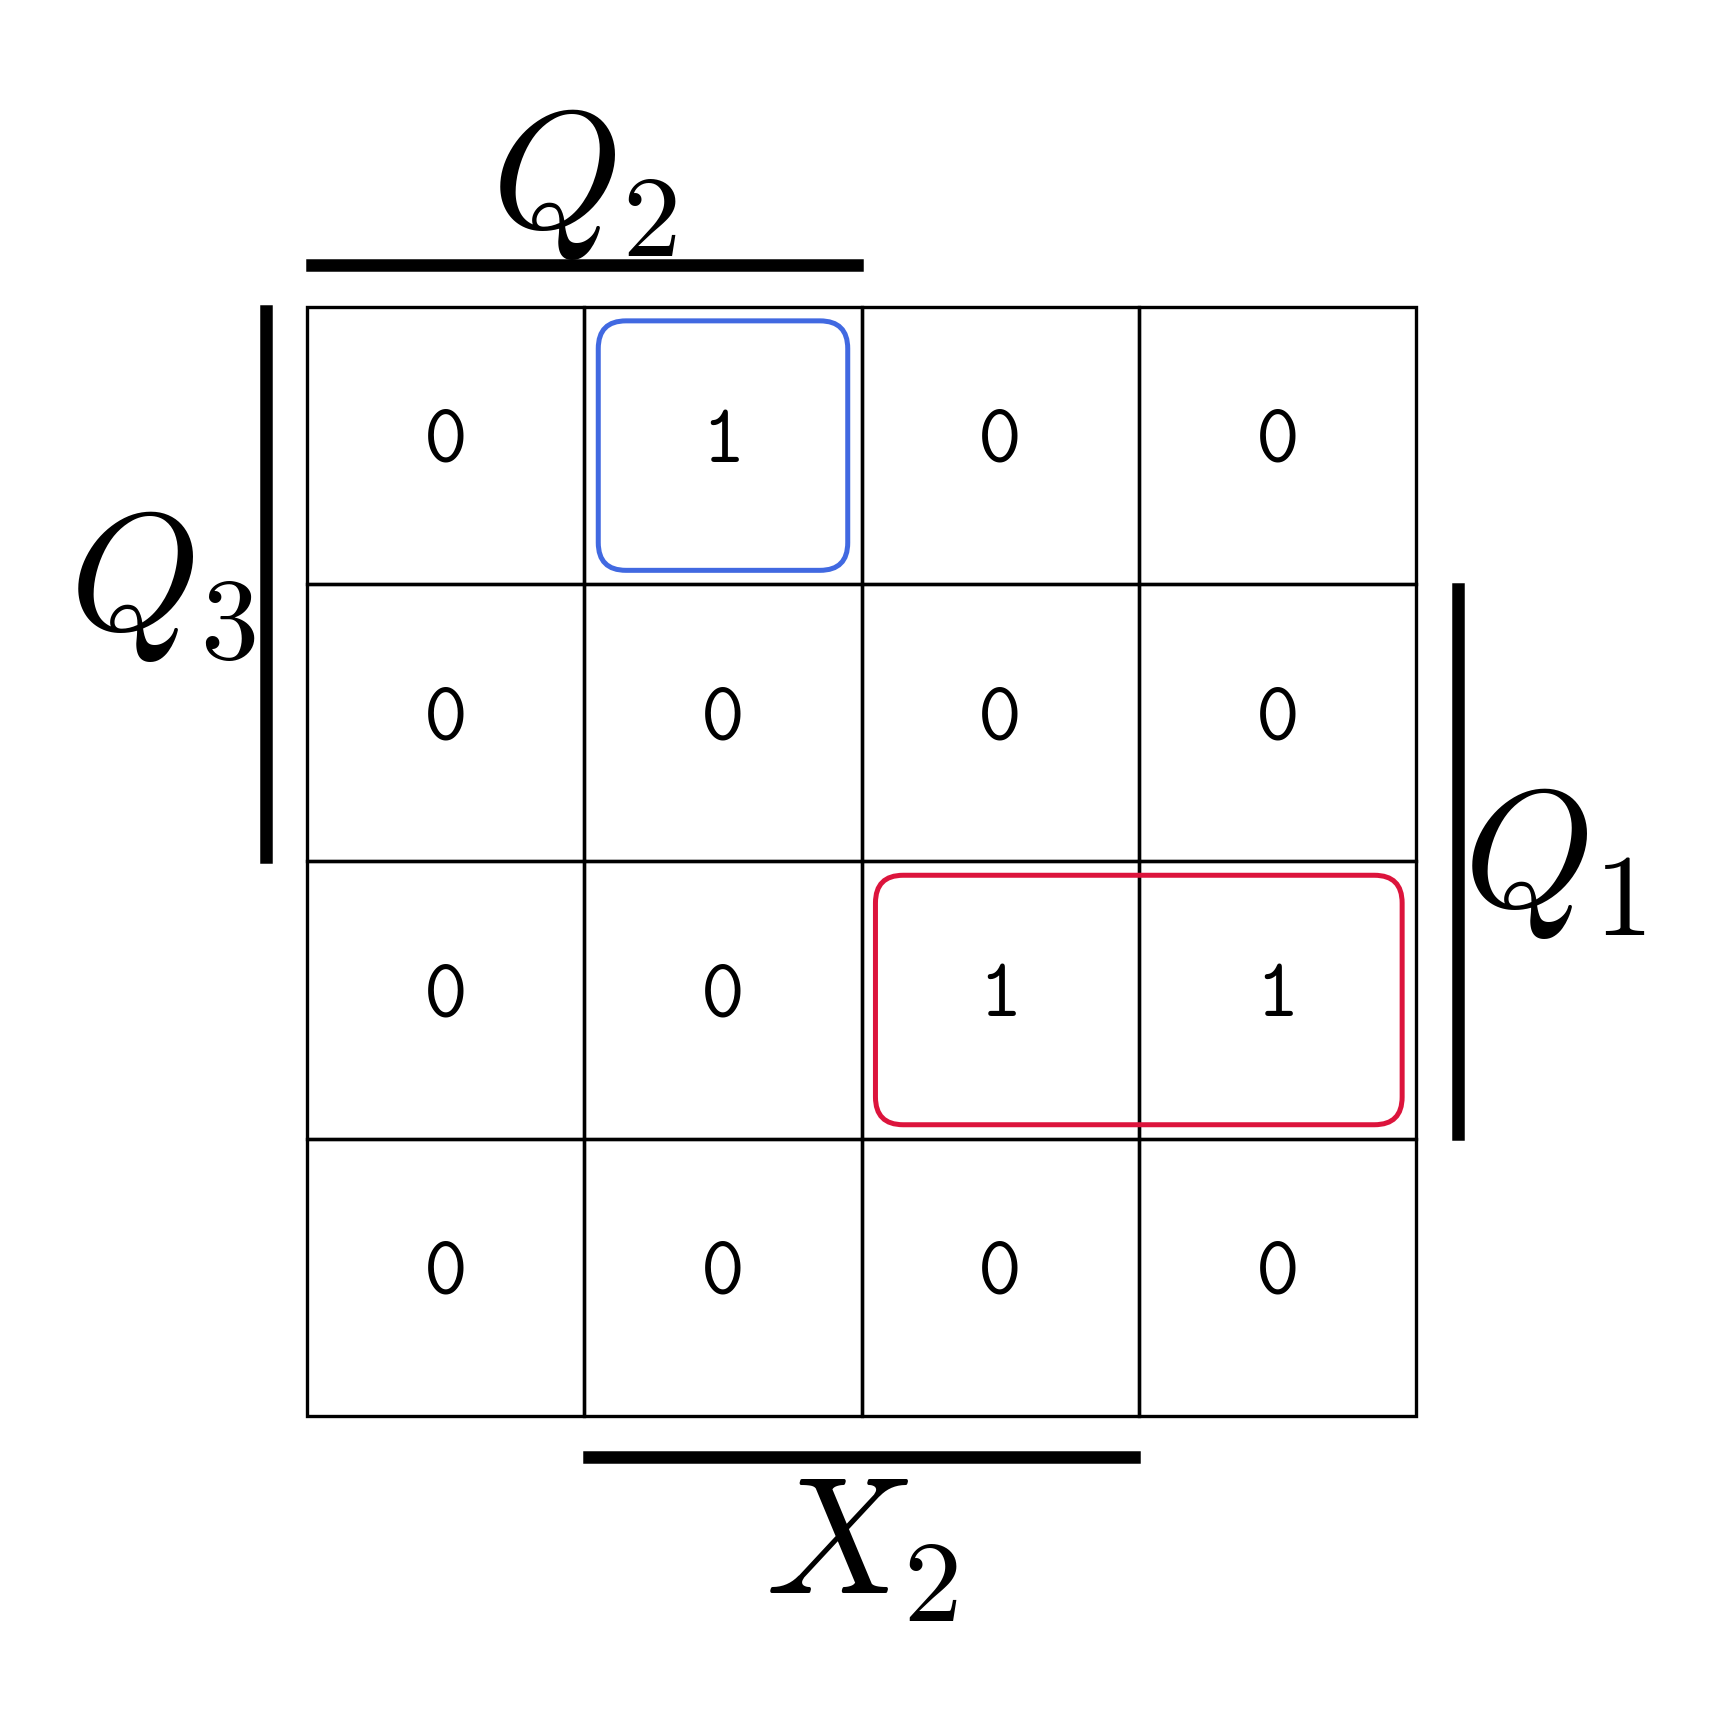
\includegraphics[width=\linewidth]{media/png files/t3.png}
            \subcaption*{а)}
        \end{subfigure}
        \hfill
        \begin{subfigure}[t]{0.3\textwidth}
            \centering
            
\includegraphics[width=\linewidth]{media/png files/t2.png}
            \subcaption*{б)}
        \end{subfigure}
        \hfill
        \begin{subfigure}[t]{0.37\textwidth}
            \centering
            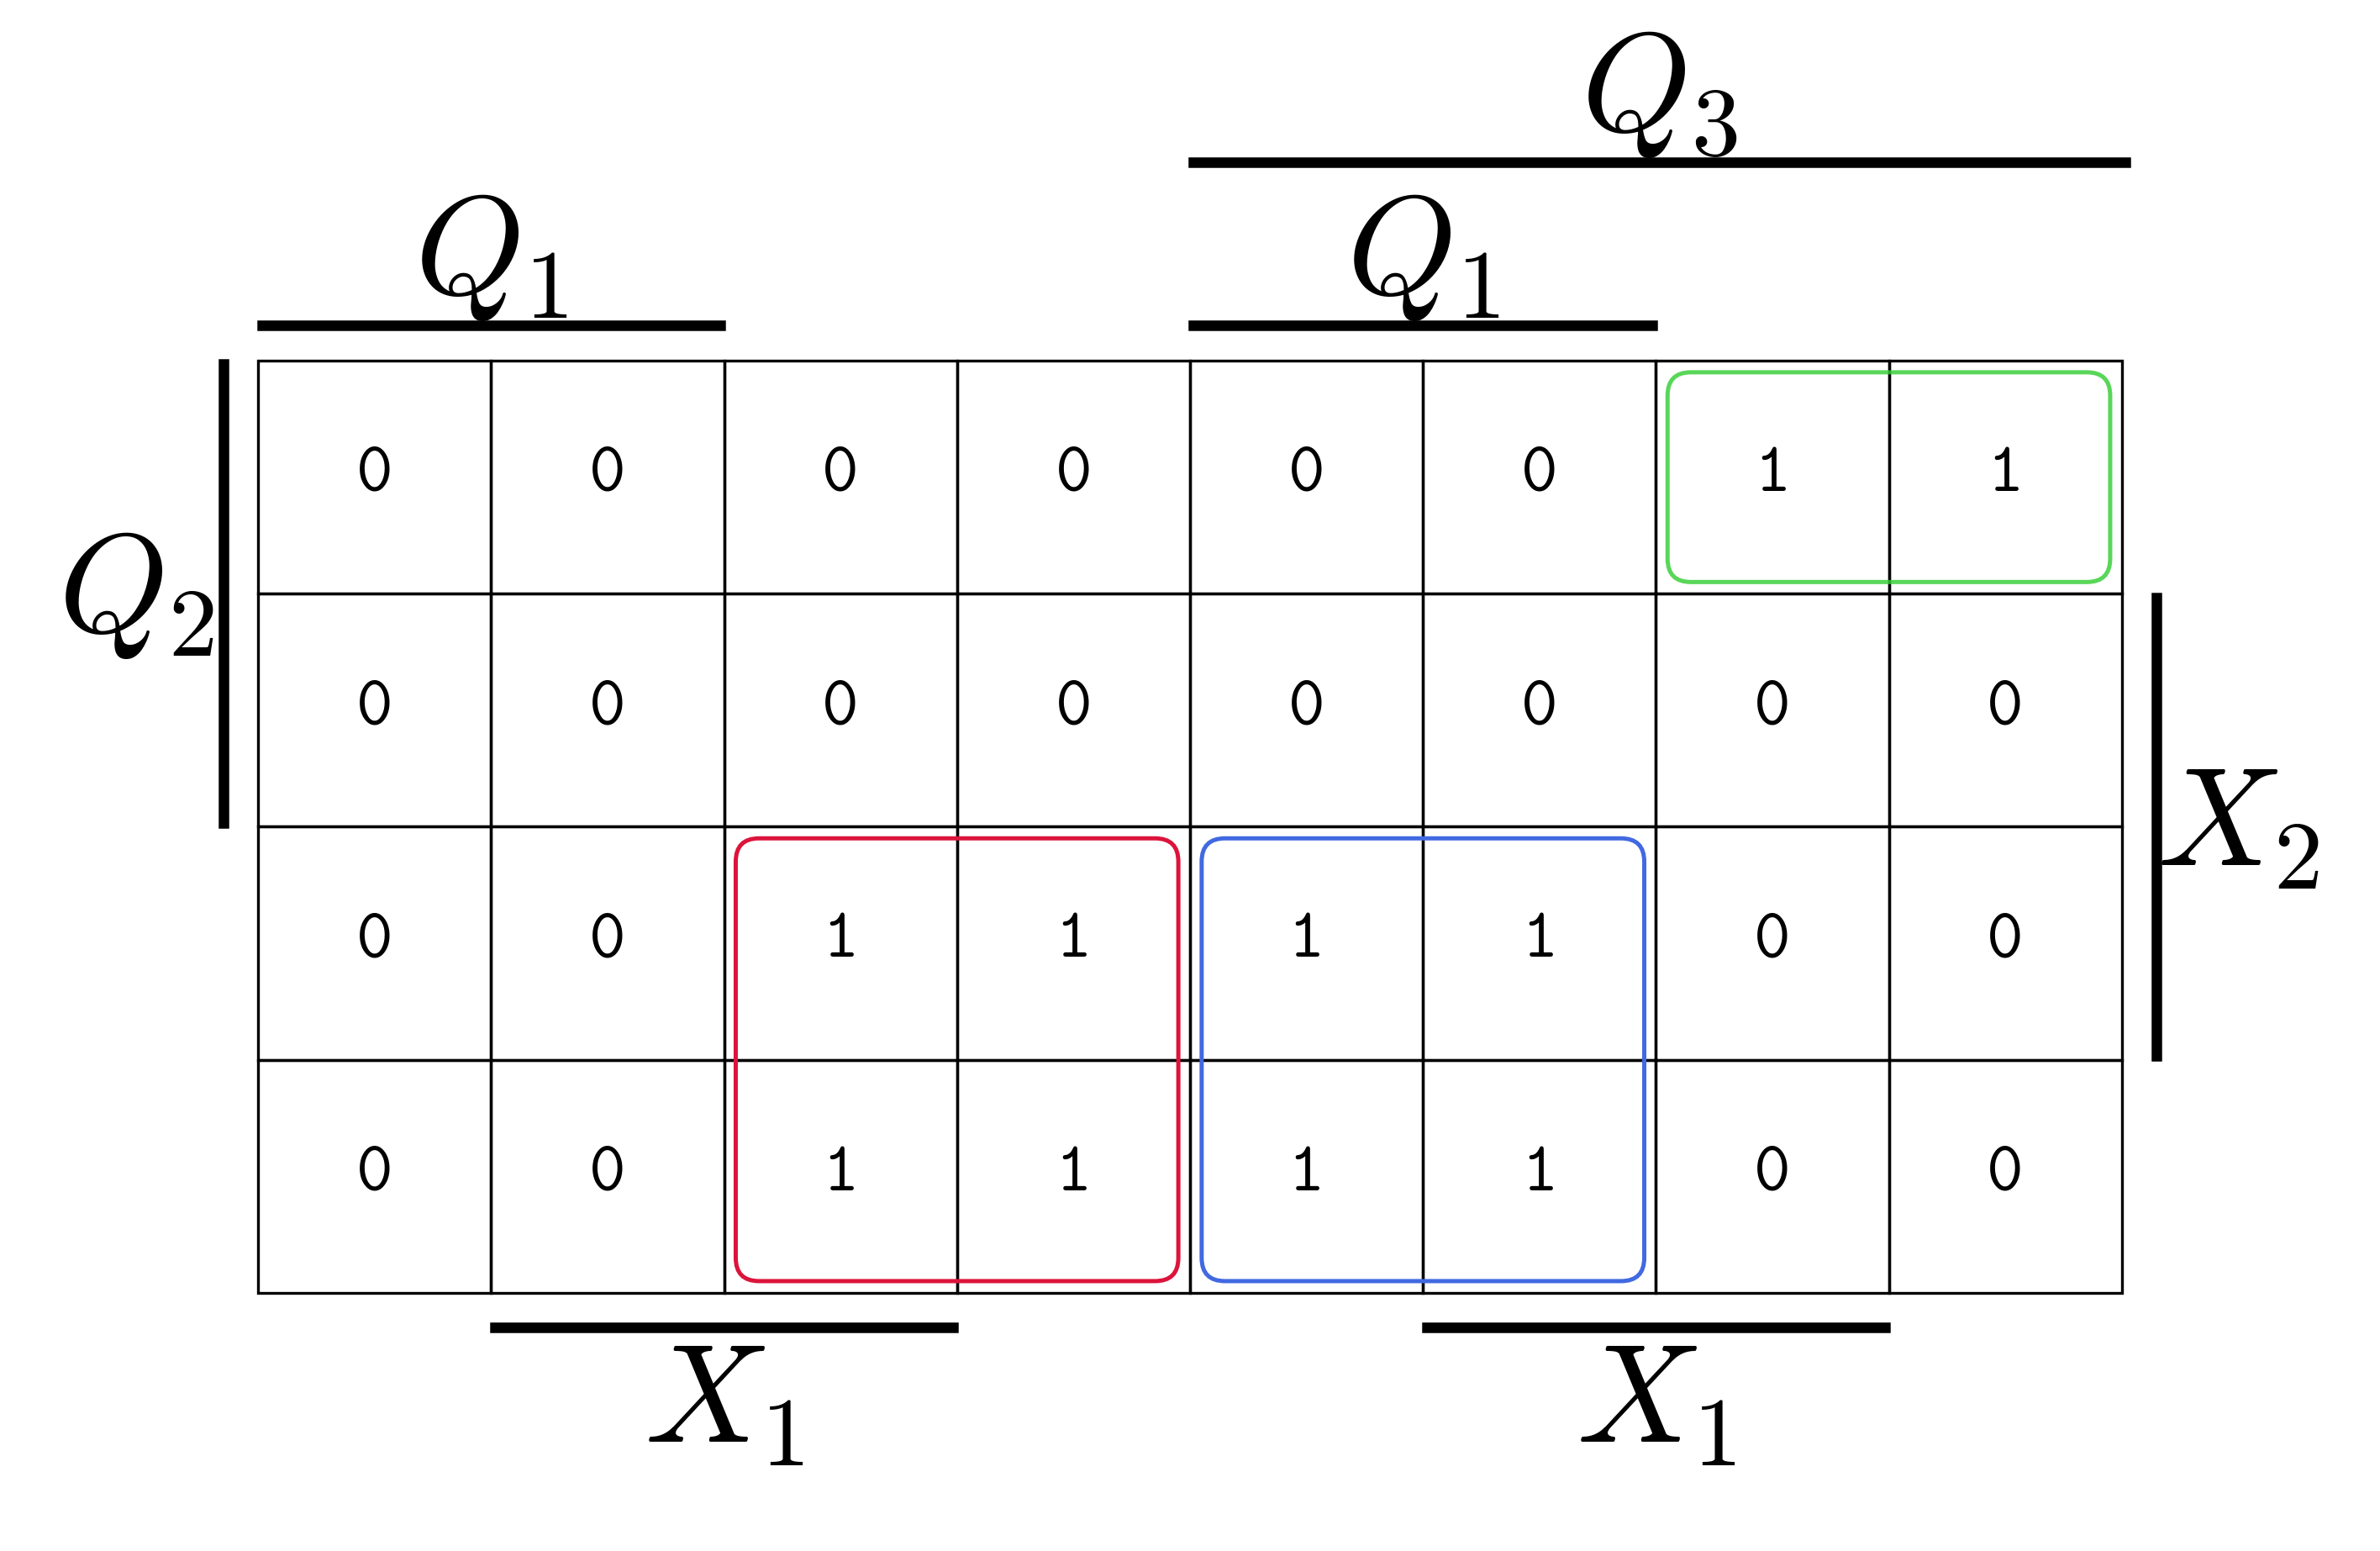
\includegraphics[width=\linewidth]{media/png files/t1.png}
            \subcaption*{в)}
        \end{subfigure}

        \caption{Діаграми Вейча для а) $T_3$, б) $T_2$, в) $T_1$}
    \end{figure}

    \noindent
    Звідси:

    \vspace{1em}

    $T_3 = \overline{Q_3} \, \overline{Q_2} \, Q_1 \vee Q_3 \, Q_2 \, \overline{Q_1} \, X_2$

    \vspace{1em}

    $T_2 = Q_3 \, \overline{Q_2} \, \overline{Q_1} \vee \overline{Q_3} \, Q_2 \, \overline{Q_1} \vee Q_3 \, Q_2 \, Q_1$

    \vspace{1em}

    $T_1 = \overline{Q_3} \, \overline{Q_2} \, \overline{Q_1} \vee Q_3 \, \overline{Q_2} \, Q_1 \vee Q_3 \, Q_2 \, \overline{Q_1}\, \overline{X_2}$

    \vspace{1em}

    \noindent
    Змоделюємо спочатку керуючий автомат, та пореревіримо його правильність, порівнюючи часові діаграми із графом:

    \begin{figure}[h!]
        \centering
        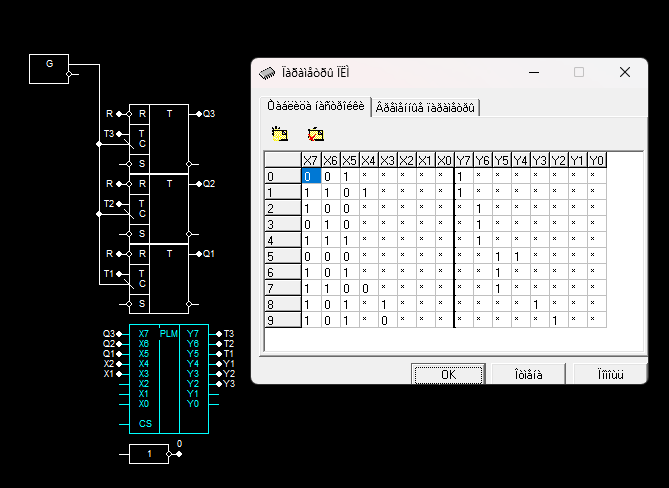
\includegraphics[width=0.7\linewidth]{media/png files/auto.png}
        \caption{\centering Схема керуючого автомата для множення 2 способом. Комбінаційна частина реалізована на ПЛМ(8; p; 8)}
    \end{figure}

    \newpage

    \noindent
    І надамо її часову діаграму:

    \begin{figure}[h!]
        \centering
        
\includegraphics[width=0.7\linewidth]{media/png files/time1.png}
        \caption{\centering Часова діаграма роботи керуючого автомата}
    \end{figure}

    Згідно із часовою діаграмою, наш автомат виконує наданий мікроалгоритм правильно, та повністю відповідає його графу.

    Тепер побудуємо операційний пристрій множення 2 способом 4-розрядних двійкових чисел:

    \begin{figure}[h!]
        \centering
        
\includegraphics[width=0.7\linewidth]{media/png files/op_scheme.png}
        \caption{\centering Схема операційного пристрою для множення 2 способом}
    \end{figure}

    \newpage

    \noindent
    Узагальнена структура арифметико-логічного пристрою:

    \begin{figure}[h!]
        \centering
        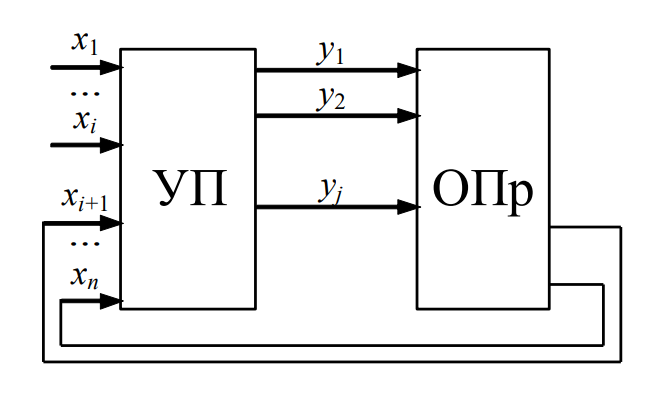
\includegraphics[width=0.7\linewidth]{media/png files/alu.png}
        \caption{\centering Узагальнена схема АЛП}
    \end{figure}

    Де $x_1, x_2, \dots, x_n$ -- вхідні дані (для нашого АЛП існують лише $x_1$ та $x_2$). Та керуючі сигнали операційним пристроєм $y_1, y_2, \dots y_i$, що
    в нашому випадку окремо існують $y_1, y_2$ та $y_3$.

    \noindent
    Тепер побудуємо АЛП множення 2 способом у програмі моделювання логічних схем AFDK:

    \begin{figure}[h!]
        \centering
        
\includegraphics[width=0.7\linewidth]{media/png files/alu_afdk.png}
        \caption{\centering Схема АЛП множення 2 способом у AFDK}
    \end{figure}

    \newpage

    І відразу перевіримо правильність виконання множення операндів $A$ та $B$ і бачимо, що множення пройшло успішно та відповідь коректна. Також надам часову діаграму АЛП:

    \begin{figure}[h!]
        \centering
        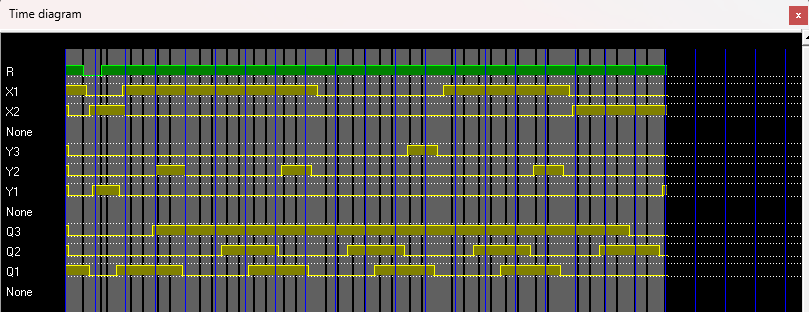
\includegraphics[width=0.7\linewidth]{media/png files/time_diagr.png}
        \caption{\centering Часова діаграма АЛП}
    \end{figure}

    Часова діаграма ще раз підтверджує коректність синтезу АЛП множення 2 способом 4-розрядних двійкових чисел
    за допомогою $T$-тригерів, що реалізують автомат Мілі.

    \begin{center} \textbf{\large Висновок} \end{center}

    У ході виконання лабораторної роботи було синтезовано арифметико-логічний пристрій з розподіленою логікою для виконання операції множення 2 способом для 4-розрядних вхідних операндів. Розроблено операційну та функціональну схеми, складено змістовний і структурний мікроалгоритми, а також виконано логічне моделювання роботи пристрою за таблицею станів регістрів, що підтвердило коректність обчислення результату множення.

    Також було здійснено синтез пристрою керування у вигляді керуючого автомата Мілі на $T$-тригерах: побудовано граф закодованого мікроалгоритму, виконано кодування станів (за кодом Грея), складено структурну таблицю, отримано та мінімізовано (за діаграмами Вейча) функції збудження тригерів і керуючі сигнали. Реалізацію операційного пристрою та керуючого автомата виконано у середовищі AFDK (ПРОГМОЛС 2.0); часові діаграми підтвердили правильність переходів станів, формування керуючих сигналів і коректну роботу АЛП у цілому. Отримані результати відповідають заданому мікроалгоритму та підтверджують досягнення мети роботи — набуття практичних навичок проектування АЛП з розподіленою логікою та автоматів керування з жорсткою логікою.

    \begin{center} \textbf{\large Відповіді на контрольні запитання} \end{center}

    \begin{enumerate}
        \item \textbf{Охарактеризуйте чотири основних методи множення чисел.}

        \textbf{1-й спосіб (зсув добутку вправо).}
        На початку кожного циклу аналізується молодший розряд множника в регістрі $RG2$ (біт $RG2[1]$).
        Якщо $RG2[1]=1$, то вміст $RG3$ додається до часткових добутків у $RG1$; якщо $RG2[1]=0$ --- додавання не виконується.
        Далі виконується правий зсув у $RG1$ і $RG2$, що еквівалентно множенню на $2^{-1}$; при цьому молодший розряд $RG1$ переноситься у старший розряд $RG2$.
        Після $n$ циклів молодші розряди добутку містяться в $RG2$, а старші --- в $RG1$.
        Максимальний час виконання:
        \[
            t_M = n\,(t_p + t_3),
        \]
        де $t_p$ --- час зсуву/пересилання, $t_3$ --- час додавання.

        \textbf{2-й спосіб (зсув доданка вліво).}
        Множник $X$ записується в $RG2$, а множене $Y$ --- у молодші розряди $RG3$.
        У кожному циклі додавання керується розрядом $RG2[1]$, а в $RG3$ виконується зсув вліво.
        Завдяки цьому зсув синхронізується з додаванням, що зменшує тривалість циклу.
        Завершення операції визначається умовою обнулення $RG2$ (це особливо корисно для ненормалізованого множника).
        Час виконання зазвичай оцінюють як
        \[
            t_M = n\,t_p.
        \]

        \textbf{3-й спосіб (формування часткового добутку зі зсувом вліво).}
        Множник $X$ записується у старші розряди $RG2$ (при цьому $RG2[1]=0$), а $RG3$ має вагу $2^{-2n}$ і подає $Y2^{-n}$.
        Підсумовування виконується за умови $RG2[n+1]=1$ із зсувом вліво в $RG1$ і $RG2$.
        Можливий перенос із $RG1$ у $RG2$ усуває повторні переноси (спрощення перенесення).
        Після $n$ циклів молодші розряди добутку перебувають у $RG1$, а старші --- у $RG2$.
        Час виконання оцінюється аналогічно 1-му способу.

        \textbf{4-й спосіб (зсув множеного вправо).}
        Множник записується в $RG2$, а множене --- у старші розряди $RG3$.
        Додавання керується розрядом $RG2[n+1]$, а в $RG3$ виконується правий зсув, еквівалентний множенню на $2^{-1}$.
        За часовими витратами спосіб аналогічний 2-му:
        \[
            t_M = n\,t_p.
        \]

        \item \textbf{Як розрахувати розрядність вузлів операційного пристрою?}

        Розрядність вузлів (регістрів, шин, суматорів, лічильників) визначається з урахуванням:
        \begin{itemize}
            \item розрядності операндів (цілої та дробової частин, якщо це дроби);
            \item максимально можливого розряду добутку/суми (щоб уникнути переповнення);
            \item необхідних службових бітів (знак, перенос, біти зсуву/вирівнювання).
        \end{itemize}
        На практиці правильність обраної розрядності перевіряють моделюванням на граничних значеннях операндів.

        \item \textbf{Визначіть поняття: операція, мікроалгоритм, мікрооперація.}

        \textbf{Операція} --- дія над даними, наприклад додавання, віднімання, множення.

        \textbf{Мікрооперація} --- елементарна дія над вмістом регістрів (або над шинами/пам'яттю), що виконується за один такт керування:
        запис, зсув, пересилання, додавання, скидання тощо.

        \textbf{Мікроалгоритм} --- впорядкована послідовність мікрооперацій і умов переходу, яка реалізує задану операцію (або машинну інструкцію).

        \item \textbf{Наведіть типи арифметико-логічних пристроїв та їх основні відмінності.}

        \begin{itemize}
            \item \textbf{Послідовні} --- виконують операції поетапно (розряд за розрядом), простіші апаратно, але повільніші.
            \item \textbf{Паралельні} --- обробляють усі біти одночасно, працюють швидше, але потребують більше апаратних ресурсів.
            \item \textbf{Комбінаторні} --- не мають пам'яті стану, виходи залежать лише від поточних входів.
            \item \textbf{З пам'яттю (послідовні з регістрами)} --- можуть зберігати проміжні результати та стан, що дає змогу реалізовувати складніші алгоритми.
        \end{itemize}

        \item \textbf{Охарактеризуйте основні етапи проектування АЛП з розподіленою логікою.}

        \begin{enumerate}
            \item Для кожної операції будують операційну схему та функціональний мікроалгоритм (Ф-мікроалгоритм).
            \item Обирають розрядність регістрів, суматорів, шин, лічильників; виконують логічне моделювання (таблиці станів, часові діаграми).
            \item Розробляють функціональну та принципову схеми операційного пристрою (ОП) із зазначенням керувальних входів.
            \item Складають структурний мікроалгоритм (С-мікроалгоритм) з урахуванням конкретної реалізації вузлів.
            \item Виконують синтез пристрою керування (керуючого автомата) та формують керувальні сигнали.
            \item Формують повну принципову/функціональну схему всього АЛП та проводять перевірку (синхронну/асинхронну).
        \end{enumerate}

        \item \textbf{Що відображує операційна схема виконання операції?}

        Операційна схема описує послідовність перетворень даних в ОП: передавання між вузлами,
        виконання обчислень (наприклад додавання), зсуви, а також фіксацію результатів у регістрах.

        \item \textbf{Що відображує функціональна схема пристрою?}

        Функціональна схема показує основні блоки (регістр(и), суматор, лічильник, комутація)
        та зв'язки між ними, тобто архітектуру пристрою без деталізації елементної бази.

        \item \textbf{У чому відмінність функціонального та структурного мікроалгоритму?}

        Функціональний мікроалгоритм задає \emph{логіку} виконання операції як послідовність мікрооперацій і умов.
        Структурний мікроалгоритм уточнює виконання з урахуванням \emph{конкретної апаратної реалізації}
        (які саме вузли та сигнали задіяні, як організовані зсуви/записи/переноси).

        \item \textbf{Напишіть вирази, що визначають закони функціонування автоматів Мілі та Мура.}

        \textbf{Автомат Мура:}
        \[
            a^{s+1} = \delta(a^{s}, x^{s}), \qquad
            y^{s+1} = \lambda(a^{s}).
        \]

        \textbf{Автомат Мілі:}
        \[
            a^{s+1} = \delta(a^{s}, x^{s}), \qquad
            y^{s+1} = \lambda(a^{s}, x^{s}).
        \]

        \item \textbf{Намалюйте узагальнену структурну схему управляючого автомата.}

        \begin{figure}[h!]
            \centering
            
\includegraphics[width=0.5\linewidth]{media/png files/1.png}
        \end{figure}

        \item \textbf{Охарактеризуйте основні етапи проектування управляючого автомата.}

        \begin{enumerate}
            \item Формують повний перелік керувальних сигналів $y_i$.
            \item Визначають тривалості сигналів, будують закодований мікроалгоритм.
            \item Розмічають стани автомата та будують граф переходів.
            \item Виконують кодування станів і визначають кількість тригерів.
            \item Синтезують логічні функції (керувальні та збудження тригерів), мінімізують їх.
            \item Реалізують схему автомата та оптимізують (за потреби).
        \end{enumerate}

        \item \textbf{Як перейти від змістовного мікроалгоритму до закодованого мікроалгоритму?}

        Потрібно замінити словесні описи мікрооперацій та умов на:
        \begin{itemize}
            \item апаратні позначення вузлів і мікрооперацій;
            \item керувальні сигнали $y_i$ (коди мікрооперацій);
            \item логічні умови $x_j$, що визначають переходи між станами.
        \end{itemize}
        Таким чином переходять від абстрактного опису процесу до опису, придатного для синтезу автомата.

        \item \textbf{Як побудувати граф автомата?}

        За закодованим мікроалгоритмом будують вершини-стани $Z_i$ та дуги-переходи.
        \begin{itemize}
            \item Для автомата Мілі: на дугах записують логічні умови та (за потреби) керувальні сигнали, що залежать від входів.
            \item Для автомата Мура: у вершинах записують керувальні сигнали стану, а на дугах --- логічні умови переходів.
        \end{itemize}

        \item \textbf{Як здійснюється оцінка (мінімізація) станів автомата?}

        Визначається мінімально необхідна кількість станів для коректного виконання заданого алгоритму,
        з урахуванням усіх необхідних відмінностей у послідовностях керувальних сигналів та умовах переходу.

        \item \textbf{Як визначити необхідну тривалість управляючих сигналів?}

        Тривалість визначається часовими параметрами елементної бази та вузлів ОП:
        затримками логічних елементів, часами встановлення/утримання тригерів, а також умовами синхронізації з тактовим генератором.
        Практично тривалість вибирають так, щоб забезпечити стабілізацію рівнів сигналів до моменту перемикання.

        \item \textbf{Від чого залежить кількість тригерів, необхідних для побудови пам'яті автомата?}

        Якщо $M$ --- кількість станів, то мінімальна кількість тригерів:
        \[
            m = \lceil \log_2 M \rceil.
        \]

        \item \textbf{Як скласти структурну таблицю автомата?}

        Кожній дузі графа відповідає рядок таблиці:
        \[
            (\text{ПС},\, Q)\;\rightarrow\;(\text{СП},\, Q'), \quad \text{умови } x_j,\quad \text{сигнали } y_i,
        \]
        де фіксують поточний стан (ПС), наступний стан (СП), значення логічних умов переходу та набір керувальних сигналів,
        а також (за типом тригерів) записують функції збудження.

        \item \textbf{Складіть таблицю переходів для JK-, RS-, T- і D-тригерів. Наведіть їх умовне графічне позначення.}

        \begin{figure}[h!]
            \centering
            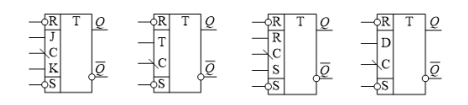
\includegraphics[width=0.5\linewidth]{media/png files/triggers.png}
        \end{figure}

        \begin{figure}[h!]
            \centering
            
\includegraphics[width=0.5\linewidth]{media/png files/2.png}
        \end{figure}

        \item \textbf{Коли можливе виникнення помилкових управляючих сигналів і чим визначається їх тривалість?}

        Помилкові короткочасні імпульси можливі під час переходів між станами через різні затримки поширення сигналів у комбінаційній логіці.
        Їх тривалість визначається різницею затримок у шляхах формування сигналів та швидкодією елементної бази.

        \item \textbf{Наведіть способи усунення короткочасних помилкових управляючих сигналів.}

        Основний підхід --- застосування сусіднього (однобітного) кодування станів (наприклад, коду Грея),
        щоб при переході змінювався лише один тригер, і тим самим зменшувалась імовірність ``тонких'' імпульсів.
        Також використовують синхронізацію сигналів, регістрацію виходів та/або введення фільтрації/затримок.

        \item \textbf{Як забезпечити перепад управляючого сигналу у випадку, коли операторну вершину з цим сигналом охоплює петля?}

        Використовують проміжний стан або додаткову затримку/формувач імпульсу,
        щоб сигнал гарантовано змінював рівень (наприклад, сформувався перепад $1\rightarrow 0$) навіть при циклічному переході (петлі).

        \item \textbf{Як визначити час переходу автомата з одного стану в інший?}

        Час переходу визначається сумою затримок комбінаційної логіки (формування збудження/виходів)
        та часових параметрів елементів пам'яті (тригерів), і узгоджується з періодом тактового сигналу (для синхронного випадку).
    \end{enumerate}









    

\end{document}